\section{Other Features}
\subsection{Collision detectors}
\red{JS}
\subsection{Integration methods}
\red{Karen}
\subsection{Lazy evaluation and automatic updating}
\label{sec:lazy}
Most kinematics libraries have a strict workflow that must be followed in order to produce correct results in a timely manner. Typically this workflow requires that all joint positions must be set and then all transforms must be computed before the transformation of a specific frame may be queried. This is a wasteful and inefficient approach for many applications.

For example, a dexterous robot manipulator may have seven links from the base to the end effector, but then it may have three fingers which each have three links. While iteratively performing inverse kinematics, it will be necessary to repeatedly compute the seven matrix transformations that go from the base to the end effector, but the transforms of the nine finger links are unnecessary. A naive approach to updating kinematics will compute all 16 transforms, even though only 7 are necessary. This means that over 56\% of the computational effort of the forward kinematics is wasted. When iteratively solving an inverse kinematics problem, the bulk of time is spent computing forward kinematics. This means that intelligently updating the forward kinematics could yield a nearly 50\% reduction in computation time for this example. Similar (and more extreme) examples could be imagined for robots with multiple limbs.

Strict workflow requirements can also lead to bugs in code. If a human programmer is not familiar with the correct workflow, does not fully understand the necessary order of operations, or simply makes a programming error, then there may be bugs in a complex controller which would produce incorrect results. Incorrect results on a dexterous manipulator could cause a task to fail and damage the robot. Incorrect results on a high-powered robot could severely damage the robot and even endanger human lives.

\subsubsection{Design}

KIDO resolves those concerns using lazy evaluation and automatic updating. Most kinematic and dynamic quantities in KIDO are automatically updated and lazily evaluated (see section \ref{sec:lazy_exception} for the exceptions). \textit{Automatic updating} means that you never need to explicitly call any kind of ``update'' function in order to get the correct output based on your most recent input. \textit{Lazy evaluation} means that expensive computations are held off until they are absolutely required by the user. Combined, these two add a decisive level of code safety to applications that use KIDO, and they cut out a considerable degree of potential waste, both while making the library easier to use. This is accomplished with the following setup:

\begin{itemize}
  \item Mutator and accessor methods (a.k.a. setters and getters) intercept all interactions with the internal states and properties of kinematic objects.
  \item Dirty flags are used to keep track of which quantities are out of date, and the dirtiness gets propagated to all dependencies.
  \item Accessor methods will check any relevant dirty flags and perform computations as necessary.
  \item Mutator methods will trigger dirty flags.
\end{itemize}

A visual example of this scheme applied to forward kinematics can be seen in figure \ref{fig:lazy}. Note that the propagation of dirty flags throughout the kinematic structure will short-circuit any time a kinematic object already knows that it is dirty. This prevents the bookkeeping from having $O(N^2)$ complexity when all $N$ joints in the kinematic structure undergo changes.

To facilitate this lazy evaluation, KIDO abides by logical const-correctness (rather than physical const-correctness). The values that are lazily evaluated are stored as mutable members of their class, allowing the \texttt{getX()} functions to be const member functions. However, because of this mutability, the const-qualifier on member functions does \textbf{not} guarantee thread-safety. Currently, the only guaranteed way to ensure thread-safety with KIDO is to spawn identical copies of the kinematic structures for each thread. This is done easily with the various \texttt{clone()} functions throughout KIDO. To spawn an identical copy of a single Skeleton, simply call \texttt{Skeleton::clone()} on it. To spawn an identical copy of a whole environment, you can use the \texttt{simulation::World::clone()} function.

\begin{figure}
  \centering
  \subfigure[][\label{fig:lazy_1}Everything is cached]{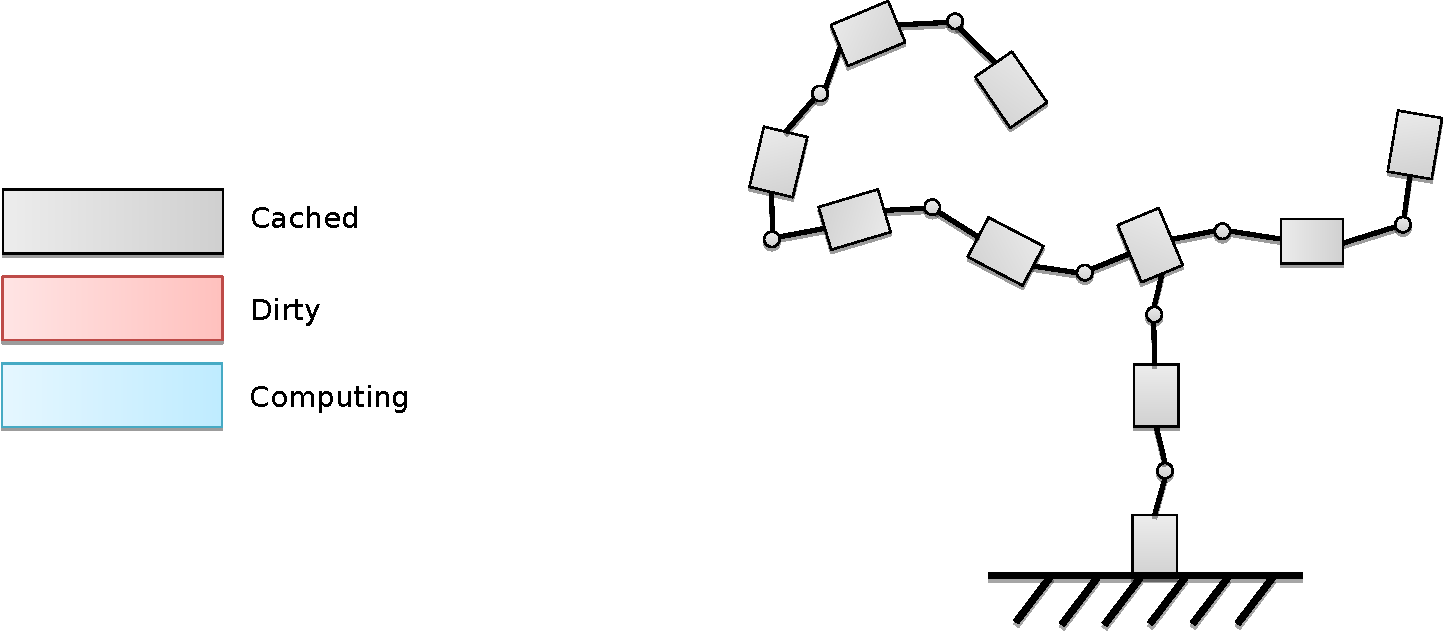
\includegraphics[width=0.98\textwidth]{fig/lazy_1.pdf}}
  
  \subfigure[][\label{fig:lazy_2}Some joint values have changed]{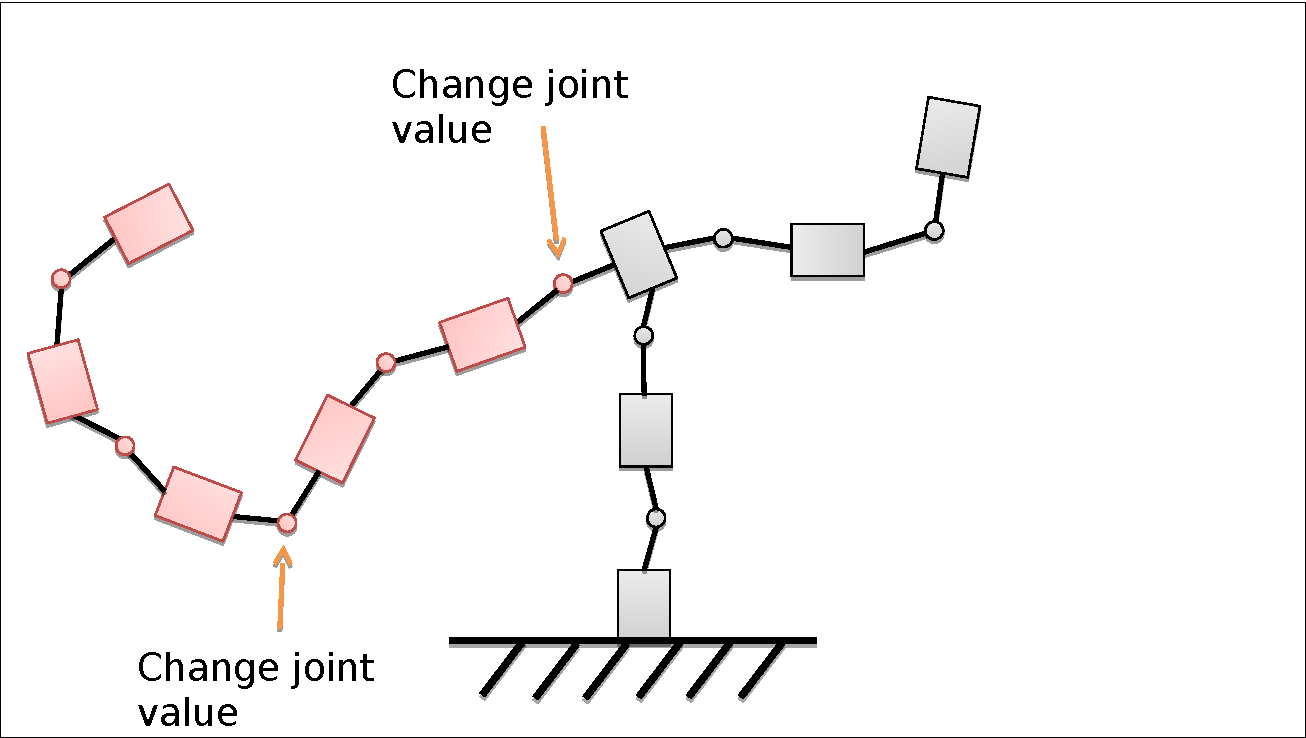
\includegraphics[width=0.44\textwidth]{fig/lazy_2.pdf}}
  \subfigure[][\label{fig:lazy_3}A dirty transform is queried]{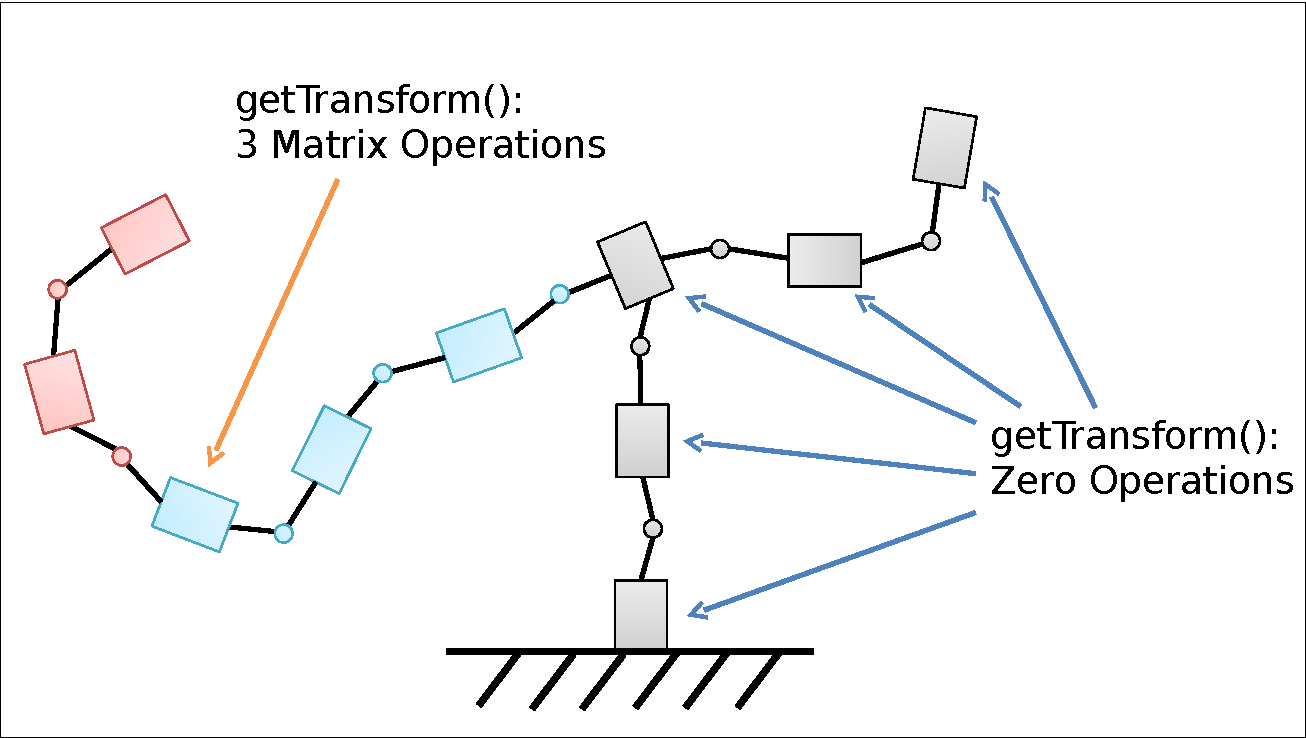
\includegraphics[width=0.44\textwidth]{fig/lazy_3.pdf}}
  
  \subfigure[][\label{fig:lazy_4}Cached transforms can be used freely]{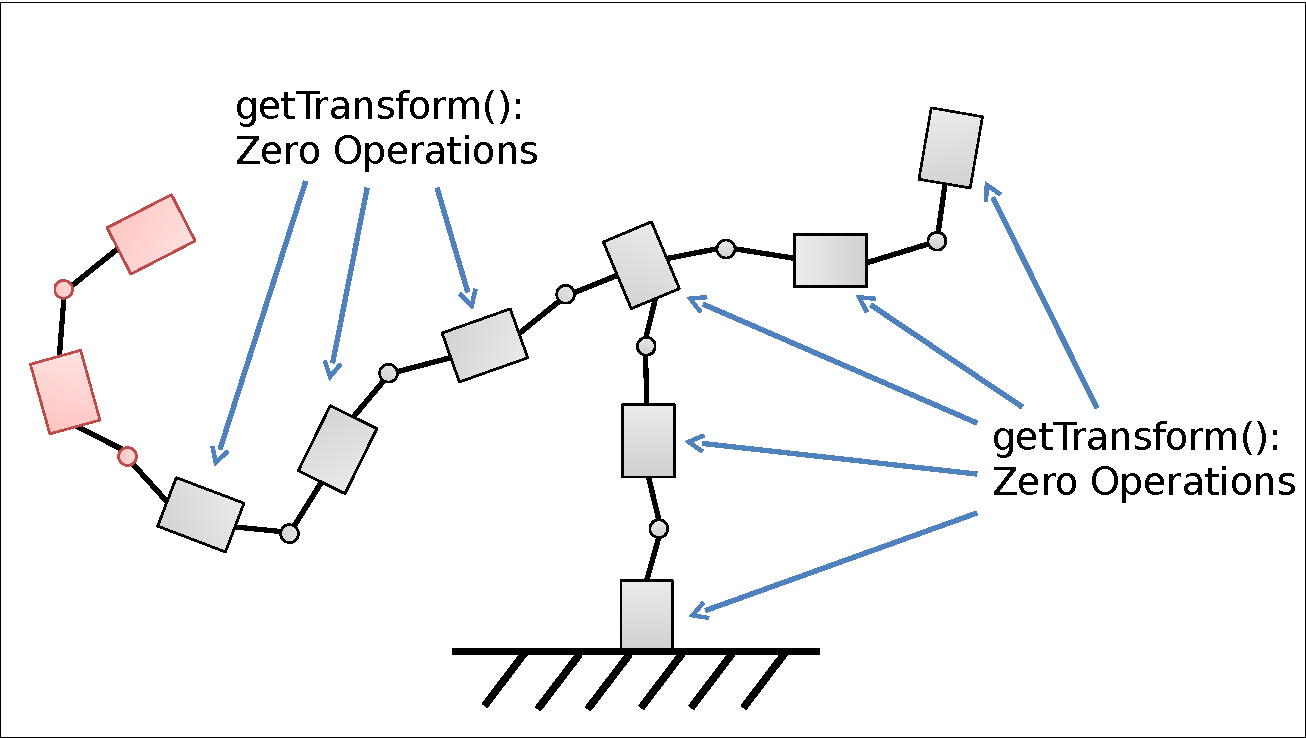
\includegraphics[width=0.44\textwidth]{fig/lazy_4.pdf}}
  \subfigure[][\label{fig:lazy_5}Another dirty transform is queried]{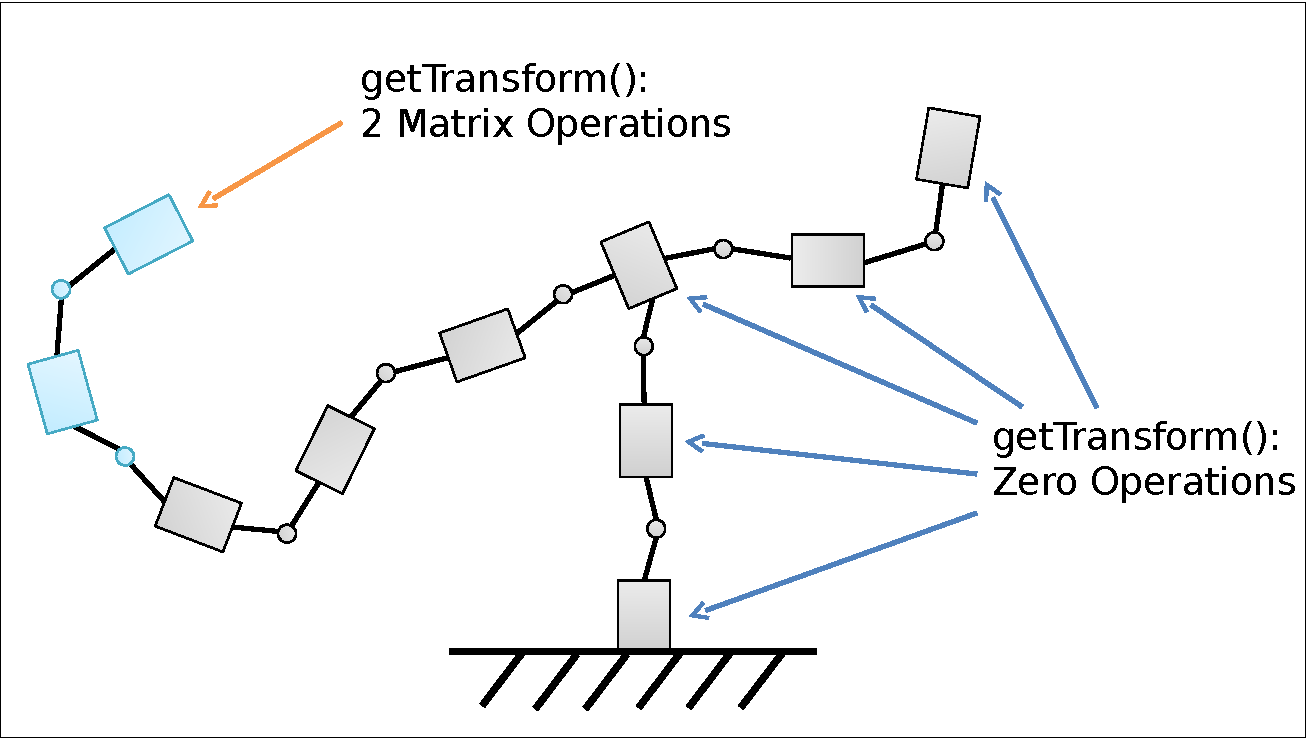
\includegraphics[width=0.44\textwidth]{fig/lazy_5.pdf}}
  \caption{Illustration of lazy evaluation for forward kinematics}
  \label{fig:lazy}
\end{figure}

In some cases, it might be undesirable to delay the computations until the time that they are requested. For example, if a real-time controller has strict scheduling requirements, there might be a specific time window which is best suited for performing heavy computations. In that case, KIDO provides a \texttt{Skeleton::computeForwardKinematics()} function which will compute all the forward kinematics within a Skeleton instead of waiting for it to be automatically updated. There are also \texttt{Skeleton::computeForwardDynamics()} and \texttt{Skeleton::computeInverseDynamics()} functions which will compute all the various dynamics parameters instead of waiting to evaluate them as needed.

\subsubsection{Exceptions: Forward and Inverse Dynamics Updating}
\label{sec:lazy_exception}
Even though forward kinematics is updated automatically, neither forward nor inverse dynamics have this quality. Individual dynamics parameters---such as the mass matrix, Coriolis forces, and articulated inertia---are updated automatically, but KIDO will \textbf{not} automatically compute the body accelerations due to the current joint torques or vice versa. This is due to the ambiguous nature of how the user might want to utilize the library: Do they want to simulate forward to see a result or compute the inverse dynamics to inform a controller? In order to compute one or the other automatically, the library would need to make an assumption about which one the user is interested in, but KIDO is meant to be suitable for both. Instead, KIDO requires the user to specifically request one or the other each time they want the results:

\begin{itemize}
  \item \textbf{\texttt{Skeleton::computeForwardDynamics()}} should be used to compute the accelerations of all the BodyNodes given the current generalized forces (or more generally, the current commands) of their joints.
  \item \textbf{\texttt{Skeleton::computeInverseDynamics()}} should be used to compute the generalized forces needed by the joints in order to achieve the current accelerations of the BodyNodes.
\end{itemize}

The results of each call will show up in the joint states of the Skeleton. The results of \texttt{computeForwardDynamics()} will show up in \texttt{Joint::getAccelerations()} and then by extension \texttt{BodyNode::getSpatialAcceleration()}, \texttt{getLinearAcceleration()}, and \texttt{getAngularAcceleration()}. The results of \texttt{computeInverseDynamics()} will show up in \texttt{Joint::getForces()} and by extension \texttt{Skeleton::getForces()}.

In both cases, the functions make use of kinematics and dynamics parameters which are cached and lazily evaluated, so making redundant calls to these functions is not prohibitively expensive, although it is still not completely free of charge.

\subsection{Extensible data structures}

There are countless applications for kinematics and dynamics software, and the developers of KIDO do not anticipate that we could possibly account for all use cases. Instead of limiting the potential applications of the library with a closed-off design, we have made the kinematics and dynamics structures extensible by introducing the concepts of \textbf{Addon}s and \textbf{Node}s.

\textbf{Addon}s and \textbf{Node}s have some practical and semantic differences, but their overarching motivation is the same: They provide a way to embed arbitrary data and functionality into kinematic and dynamic structures. For example, if you want to have a custom sensor type that can be attached to a body on your robot, you could create a custom \textbf{Node} and attach instances of your \textit{SensorNode} on whichever bodies need it.

Any concept can be encapsulated into either an \textbf{Addon} or a \textbf{Node} as long as its contents can be decomposed into a \textbf{State} structure and/or a \textbf{Properties} structure (or neither if the concept contains no information at all). To fully understand whether an Addon or a Node should be used for your purposes, the following subsections will explain the difference, but the differences can be boiled down to these:

\begin{itemize}
  \item A \textbf{BodyNode} can only contain a single instance of any particular type of \textbf{Addon}, but it can contain arbitrarily many of any particular type of \textbf{Node}.
  \item \textbf{Node}s can only be attached to \textbf{BodyNode}s, but \textbf{Addon}s can be attached to any class that inherits \textbf{AddonManager} (e.g. \textbf{Joint}, \textbf{Skeleton}, \textbf{EndEffector}).
\end{itemize}

\subsubsection{Addons}
\label{sec:addons}

There may be times where you have developed a novel algorithm that requires extra contextual information that might not be natively available in KIDO. For example, you might have computed an occupancy grid for some geometry, but KIDO does not natively support occupancy grids. Nevertheless, you want the information to be embedded in the geometric object; you want it to be saved as part of the object's \textbf{Properties}, and you want it to get copied over whenever the object is cloned.

You could achieve this by defining an \textit{OccupancyGrid} class that inherits the \textbf{Addon} class. Then you could embed an instance of an \textit{OccupancyGrid} class into the \textbf{ShapeNode} instance that holds the geometric data for which the occupancy grid was calculated:

\begin{lstlisting}
shapeNode->create<OccupancyGrid>(gridInfo);
\end{lstlisting}

You can then retrieve it with:

\begin{lstlisting}
OccupancyGrid* grid = shapeNode->get<OccupancyGrid>();
\end{lstlisting}

If the \texttt{shapeNode} instance has never been given or created an \texttt{OccupancyGrid} object, this function will return a \texttt{nullptr} by default. It is always a good idea to check whether the \textbf{Addon} pointer that gets returned is a \texttt{nullptr}, because KIDO does not throw any exceptions or assertions when you request an \textbf{Addon} that is not present in the object.

\subsubsection{Nodes}
\label{sec:nodes}
\red{Grey}
\subsection{History recorder}
\todo[MXG]{It doesn't look like we'll have this in time for the next major release, although it will probably be available for the next minor release. Will it be possible to update this tech report as we add features and make changes?}
\subsection{Optimization interface}
\label{sec:optimizer}
\red{Grey}
\subsection{Extensible GUI}
\red{JS}
